% ============================================================
%  Campus Cloud Print Queue — CS 6650 Final Project Report
%  Team: Anand Mohan Singh, Vaibhav Thalanki, Pranav Viswanathan
%  Northeastern University · April 2026
% ============================================================
\documentclass[11pt,letterpaper]{article}

% ── Packages ─────────────────────────────────────────────────
\usepackage[margin=1in]{geometry}
\usepackage{graphicx}
\usepackage{booktabs}
\usepackage{array}
\usepackage{tabularx}
\usepackage{multirow}
\usepackage{xcolor}
\usepackage{hyperref}
\usepackage{enumitem}
\usepackage{fancyhdr}
\usepackage{titlesec}
\usepackage{parskip}
\usepackage{microtype}
\usepackage{listings}
\usepackage{caption}
\usepackage{subcaption}
\usepackage{float}
\usepackage{mdframed}
\usepackage{fontawesome5}
\usepackage{amsmath}
\usepackage{amssymb}
\usepackage{tcolorbox}
\usepackage{pgfplots}
\usepackage{pgfplotstable}
\usepackage{tikz}
\usetikzlibrary{shapes.geometric, arrows.meta, positioning, fit, backgrounds, calc}
\pgfplotsset{compat=1.18}

% ── Colors ───────────────────────────────────────────────────
\definecolor{primary}{HTML}{1E40AF}    % deep blue
\definecolor{accent}{HTML}{F59E0B}     % amber
\definecolor{success}{HTML}{059669}    % emerald
\definecolor{danger}{HTML}{DC2626}     % red
\definecolor{surface}{HTML}{F1F5F9}    % light gray-blue
\definecolor{codebg}{HTML}{1E293B}     % dark slate
\definecolor{codefg}{HTML}{E2E8F0}     % light text
\definecolor{muted}{HTML}{64748B}      % slate-500
\definecolor{border}{HTML}{CBD5E1}     % slate-300
\definecolor{section-rule}{HTML}{3B82F6}

% ── Hyperref ─────────────────────────────────────────────────
\hypersetup{
  colorlinks=true,
  linkcolor=primary,
  urlcolor=primary,
  citecolor=primary,
  pdftitle={Campus Cloud Print Queue -- CS 6650 Final Report},
  pdfauthor={Anand Mohan Singh, Vaibhav Thalanki, Pranav Viswanathan},
}

% ── Section formatting ───────────────────────────────────────
\titleformat{\section}
  {\large\bfseries\color{primary}}
  {\thesection.}{0.6em}{}
  [\color{section-rule}\rule{\linewidth}{1.5pt}]

\titleformat{\subsection}
  {\normalsize\bfseries\color{primary!85!black}}
  {\thesubsection}{0.5em}{}

\titleformat{\subsubsection}
  {\normalsize\bfseries\color{muted}}
  {\thesubsubsection}{0.5em}{}

% ── Code listings ────────────────────────────────────────────
\lstset{
  backgroundcolor=\color{codebg},
  basicstyle=\tiny\ttfamily\color{codefg},
  keywordstyle=\color{accent}\bfseries,
  commentstyle=\color{muted},
  stringstyle=\color{success!70!white},
  breaklines=true,
  frame=none,
  xleftmargin=8pt,
  xrightmargin=8pt,
  aboveskip=6pt,
  belowskip=6pt,
  numbers=none,
  rulecolor=\color{border},
}

% ── tcolorbox styles ─────────────────────────────────────────
\tcbuselibrary{skins,breakable}

\newtcolorbox{claimbox}{
  colback=primary!6,
  colframe=primary!40,
  boxrule=0.6pt,
  arc=2pt,
  left=8pt, right=8pt, top=5pt, bottom=5pt,
  fonttitle=\small\bfseries\color{primary},
  title=Design Claim Under Test,
}

\newtcolorbox{resultbox}{
  colback=success!8,
  colframe=success!45,
  boxrule=0.6pt,
  arc=2pt,
  left=8pt, right=8pt, top=5pt, bottom=5pt,
  fonttitle=\small\bfseries\color{success!70!black},
  title=Result,
}

\newtcolorbox{limitbox}{
  colback=accent!7,
  colframe=accent!40,
  boxrule=0.6pt,
  arc=2pt,
  left=8pt, right=8pt, top=5pt, bottom=5pt,
  fonttitle=\small\bfseries\color{accent!80!black},
  title=Limitations,
}

% ── Header / Footer ──────────────────────────────────────────
\pagestyle{fancy}
\fancyhf{}
\fancyhead[L]{\small\color{muted}Campus Cloud Print Queue}
\fancyhead[R]{\small\color{muted}CS 6650 Final Report --- Northeastern University}
\fancyfoot[C]{\small\color{muted}\thepage}
\renewcommand{\headrulewidth}{0.4pt}
\renewcommand{\headrule}{\color{border}\hrule}

% ── Misc helpers ─────────────────────────────────────────────
\newcommand{\code}[1]{\texttt{\small #1}}
\newcommand{\http}[1]{\textbf{\texttt{#1}}}
\newcommand{\kv}[2]{\textbf{#1:} #2\par}
\setlength{\parskip}{5pt}

% ============================================================
\begin{document}

% ── Title Page ───────────────────────────────────────────────
\begin{titlepage}
\thispagestyle{empty}
% Draw the header bars as a background — text flows normally below them
\noindent
\begin{tikzpicture}[remember picture, overlay]
  \fill[primary] (current page.north west) rectangle
    ([yshift=-4.2cm]current page.north east);
  \fill[accent] ([yshift=-4.2cm]current page.north west) rectangle
    ([yshift=-4.5cm]current page.north east);
\end{tikzpicture}

% White title text sits inside the blue bar
\vspace*{0.9cm}
{\color{white}\fontsize{28}{34}\selectfont\bfseries Campus Cloud Print Queue\par}
\vspace{0.25cm}
{\color{accent!70!white}\fontsize{13}{20}\selectfont
  \textbf{Campus Print} \par}
\vspace{0.15cm}
{\color{white!75!primary}\normalsize
  CS 6650  \textperiodcentered{}
  Building Scalable Distributed Systems \textperiodcentered{}
  Final Project Report\par}

% Gap between bar bottom (4.5cm from top) and the cards
\vspace{1.6cm}

% Team card
\begin{tcolorbox}[
  colback=surface,
  colframe=border,
  boxrule=0.8pt,
  arc=4pt,
  width=1.0\textwidth,
  left=14pt, right=14pt, top=10pt, bottom=10pt,
]
  {\small\bfseries\color{muted}\MakeUppercase{Team Members}\par}
  \vspace{6pt}
  \begin{tabularx}{\linewidth}{@{}lX@{}}
    \textbf{Anand Mohan Singh}    & Infrastructure (Terraform, 9 modules), CI/CD, resilience migration, unit tests \\[3pt]
    \textbf{Vaibhav Thalanki}     & API development (Go Gin, DynamoDB schema, concurrency logic) \\[3pt]
    \textbf{Pranav Viswanathan}   & Printer worker, experiment scripts, CloudWatch observability \\
  \end{tabularx}
\end{tcolorbox}

\vspace{0.8cm}

\begin{tcolorbox}[
  colback=surface,
  colframe=border,
  boxrule=0.8pt,
  arc=4pt,
  width=0.82\textwidth,
  left=14pt, right=14pt, top=8pt, bottom=8pt,
]
  {\small\bfseries\color{muted}\MakeUppercase{Repository}\par}
  \vspace{4pt}
  \url{https://github.com/anandms101/Campus-Cloud-Print-Queue}
\end{tcolorbox}

\vfill

\begin{tcolorbox}[
  colback=primary!5,
  colframe=primary!25,
  boxrule=0.6pt,
  arc=3pt,
  width=0.82\textwidth,
  left=12pt, right=12pt, top=7pt, bottom=7pt,
]
  {\small\bfseries\color{muted}\MakeUppercase{Deliverable Index}\par}
  \vspace{4pt}
  \begin{tabular}{@{}lll@{}}
    \S1 & Video Presentation      & 5 marks \\
    \S2 & Code and Repository     & 5 marks \\
    \S3 & Project Management      & 5 marks \\
    \S4 & Experiments Report      & 10 marks \\
    \S5 & Community Contributions & 5 marks \\
  \end{tabular}
\end{tcolorbox}
\end{titlepage}

% ── Table of Contents ────────────────────────────────────────
\tableofcontents
\newpage

% ============================================================
\section{Video Presentation}
\label{sec:video}

The submission includes one screen-capture video in which each team member presents the portion of the project they personally built. The video is segmented as follows.

\subsection{Segment 1 --- Vaibhav Thalanki}
Vaibhav presents the Go Gin API service: the seven endpoint handlers, the DynamoDB conditional expression logic used for every state transition, the GSI schema design (\code{userId-createdAt-index}), middleware layering (request ID, structured logging, timeout, rate limiter), the circuit breaker configuration via \code{sony/gobreaker/v2}, and the bulkhead semaphore around the upload handler. He also demonstrates and explains the Bulkhead isolation applied to the \http{POST /jobs} endpoint in the Go Gin implementation.

\subsection{Segment 2 --- Anand Mohan Singh }
Anand walks through the infrastructure layer: the nine Terraform modules (\code{networking}, \code{ecr}, \code{iam}, \code{dynamodb}, \code{s3}, \code{sqs}, \code{alb}, \code{ecs}, \code{cloudwatch}), the use of \code{for\_each} over the \code{printer\_names} variable to instantiate per-printer SQS queues and ECS services, and the Makefile automation (\code{make deploy-fresh}, \code{make teardown}, \code{make queue-depth}, etc.). He demonstrates a live \code{terraform plan} output and shows the CloudWatch dashboard with all six panels active.

\subsection{Segment 3 --- Pranav Viswanathan (2--3 minutes)}
Pranav covers the Python printer worker: the SQS long-polling loop, the idempotency state machine in \code{processor.py} including the crash recovery branch (\code{status=PROCESSING} and \code{receiveCount > 1}), the visibility-extension heartbeat, and the compensating logic for S3 download failures. He then walks through all four experiment scripts (\code{locustfile.py}, \code{contention\_test.py}, \code{saturation\_test.py}, \code{fault\_injection\_test.py}) and the CloudWatch log group and dashboard configuration.

\medskip
\begin{tcolorbox}[
  colback=surface,
  colframe=border,
  boxrule=0.6pt,
  arc=2pt,
  left=8pt, right=8pt, top=5pt, bottom=5pt,
]
  \textbf{Video link:} \url{https://youtu.be/W4ehZsmXToc}
\end{tcolorbox}


% ============================================================
\section{Code and Repository}
\label{sec:code}

\subsection{Primary Repository}
\url{https://github.com/anandms101/Campus-Cloud-Print-Queue}

The repository was developed collaboratively with commits from all three team members. Commit history, branch activity, and issue tracking reflect the progression of the project from initial architecture through final experiment execution.

\subsection{README Overview}
The \code{README.md} introduces the project motivation (release-at-device printing), explains the system architecture at a high level with a diagram, and provides a quickstart guide covering prerequisites, environment variable setup, and the single-command deployment (\code{make deploy-fresh}). It links to the architecture documentation in \code{docs/ARCHITECTURE.md} and includes \code{curl} examples for all six API endpoints.

\subsection{Repository Structure}

\begin{lstlisting}[language=bash]
Campus-Cloud-Print-Queue/
+-- Makefile                           # All operational commands (deploy, test, logs, teardown)
+-- README.md
+-- services/
|   +-- api-gin/
|   |   +-- main.go                    # HTTP server, graceful shutdown
|   |   +-- handlers.go                # 7 endpoint handlers
|   |   +-- models.go                  # JobItem struct (DynamoDB + JSON)
|   |   +-- config.go                  # Env var loading + validation
|   |   +-- middleware.go              # Request ID, logger, timeout, rate limiter
|   |   +-- resilience.go              # Circuit breaker factory
|   |   +-- interfaces.go              # DynamoAPI, S3API, SQSAPI
|   |   +-- handlers_test.go           # 25 unit tests
|   |   +-- mocks_test.go              # Mock AWS interfaces
|   |   +-- Dockerfile                 # Multi-stage Go build (~15 MB image)
|   +-- printer-worker/
|       +-- app/
|       |   +-- main.py                # Poll loop, signal handling, backoff
|       |   +-- processor.py           # Job state machine (idempotency, crash recovery)
|       |   +-- config.py              # Env var loading
|       |   +-- services/
|       |       +-- dynamodb.py        # mark_processing, mark_done, mark_failed
|       |       +-- sqs.py             # receive, delete, visibility extension
|       |       +-- s3.py              # download, delete
|       +-- Dockerfile
|       +-- requirements.txt
+-- infra/
|   +-- main.tf
|   +-- variables.tf
|   +-- outputs.tf
|   +-- modules/
|       +-- networking/ ecr/ iam/ dynamodb/ s3/ sqs/ alb/ ecs/ cloudwatch/
+-- tests/
|   +-- unit/
|   +-- experiment1_load_test/
|   +-- experiment2_contention/
|   +-- experiment3_saturation/
|   +-- experiment4_fault_injection/
+-- docs/
+-- .github/workflows/ci.yml
\end{lstlisting}

\subsection{CI Pipeline}
Every push and pull request to \code{main} triggers four parallel GitHub Actions jobs:
\begin{enumerate}[noitemsep]
  \item \textbf{api-checks}: \code{go vet}, \code{go build}, 25 unit tests with the \code{-race} detector.
  \item \textbf{python-checks}: worker import check, 10 \code{pytest} tests backed by \code{moto}.
  \item \textbf{terraform-checks}: \code{fmt -check}, \code{init}, \code{validate}.
  \item \textbf{docker-build}: Builds both container images (does not push to ECR).
\end{enumerate}

\subsection{Testing Coverage}
The Go unit test suite (\code{handlers\_test.go}, 25 tests) exercises all seven endpoints against mock AWS interfaces defined in \code{mocks\_test.go}. Cases include happy paths, validation errors, 409 conflict paths, bulkhead enforcement, circuit breaker state transitions, compensating rollbacks, and rate limiter rejection. The Python worker test suite (\code{test\_worker.py}, 10 tests) uses \code{moto} to simulate DynamoDB, S3, and SQS in-process, covering the normal flow, duplicate suppression, S3 failure handling, and crash recovery reprocessing. \\ \\ \\


% ============================================================
\section{Project Management}
\label{sec:pm}

\subsection{Project Board}
We tracked all work through a GitHub Projects Kanban board with five columns: \textbf{Backlog}, \textbf{Ready}, \textbf{In Progress}, \textbf{In Review}, and \textbf{Done}. The board contains 20 issues --- all 20 are now closed and in the Done column. Four pull requests were merged over the course of the project, each linked to one or more issues. Every issue was assigned to at least one team member, and experiments were co-assigned to the pair who executed them together.

\medskip
\url{https://github.com/users/anandms101/projects/4}

\begin{figure}[H]
\centering

\includegraphics[width=\linewidth]{../public/GithubProject.png}
\caption{GitHub Projects board snapshot --- all 20 issues in the Done column, spanning infrastructure, API development, printer workers, four experiments, CI/CD, testing, documentation, and the final report.}
\end{figure}

\subsection{Work Breakdown by Team Member}

\begin{table}[H]
\centering
\caption{Responsibility Matrix (GitHub issue references in parentheses)}
\begin{tabularx}{\linewidth}{@{}lXcc@{}}
\toprule
\textbf{Area} & \textbf{Description} & \textbf{Owner} & \textbf{Status} \\
\midrule
Infra \& Terraform (\#9, \#5) & 9 modules (VPC, ECR, IAM, DynamoDB, S3, SQS, ALB, ECS, CloudWatch), Makefile with 20+ targets & Anand & \textcolor{success}{Done} \\
CI/CD Pipeline (\#13)   & 4-job GitHub Actions: go vet, pytest, terraform validate, docker build & Anand & \textcolor{success}{Done} \\
CloudWatch (\#16)        & 6-panel dashboard, log groups (7-day retention), structured JSON logging & Anand & \textcolor{success}{Done} \\
Load Test Graphs (\#15)  & Locust result analysis, latency percentile charts for Experiment 1 & Anand & \textcolor{success}{Done} \\
Go Gin API (\#7, \#6)    & 7 handlers, middleware, circuit breaker, bulkhead, rate limiter & Vaibhav & \textcolor{success}{Done} \\
Go Gin Resilience (PR \#20) & Migrate to Go Gin as sole API with full resilience patterns & Anand & \textcolor{success}{Done} \\
FastAPI variant (\#8)    & Python API alternative with Bulkhead isolation on POST /jobs & Vaibhav & \textcolor{success}{Done} \\
DynamoDB schema          & Table, GSI (\code{userId-createdAt-index}), TTL, conditional expressions & Vaibhav & \textcolor{success}{Done} \\
S3 cleanup (PR \#1)      & Delete S3 objects after job processing completes & Vaibhav & \textcolor{success}{Done} \\
Printer worker (\#10)    & SQS poll loop, idempotency state machine, heartbeat, S3 download & Pranav & \textcolor{success}{Done} \\
Unit tests (\#12)        & 25 Go tests (mocks) + 10 Python tests (moto); 29 total with race detector & Anand + Pranav & \textcolor{success}{Done} \\
Experiment scripts (\#4) & Locust (Exp 1, PR \#3), asyncio (Exp 2), requests (Exp 3), AWS CLI (Exp 4) & Pranav + Vaibhav & \textcolor{success}{Done} \\
Contention Exp (\#17)    & DynamoDB conditional-write concurrency validation at N=2--50 & Pranav + Vaibhav & \textcolor{success}{Done} \\
Saturation Exp (\#18)    & 50-job single-printer overload; queue drain and latency measurement & Pranav + Vaibhav & \textcolor{success}{Done} \\
Fault Injection Exp (\#19) & ECS task kill, SQS redelivery, idempotent recovery for 8 jobs & Pranav + Vaibhav & \textcolor{success}{Done} \\
Architecture docs (\#14) & System diagrams, \code{ARCHITECTURE.md}, README & All & \textcolor{success}{Done} \\
Final report (\#11)      & This document: experiments analysis, graphs, and writeup & All & \textcolor{success}{Done} \\
\bottomrule
\end{tabularx}
\end{table}

\subsection{Project Timeline}

\begin{table}[H]
\centering
\caption{Sprint Plan and Execution}
\begin{tabularx}{\linewidth}{@{}llXl@{}}
\toprule
\textbf{Week} & \textbf{Dates} & \textbf{Focus} & \textbf{Status} \\
\midrule
1 (expedited) & Mar 23--29 & Architecture finalization, AWS setup, Terraform modules & \textcolor{success}{Done} \\
1 (expedited) & Mar 23--29 & Core flow: upload, release, process; DynamoDB + SQS integration & \textcolor{success}{Done} \\
1 (expedited) & Mar 23--29 & Correctness: conditional writes, idempotent workers, error handling & \textcolor{success}{Done} \\
2             & Apr 1--7   & All 4 experiments executed, metrics collected, graphs produced & \textcolor{success}{Done} \\
3             & Apr 8--15  & Final analysis, report writing, video recording, presentation prep & \textcolor{success}{Done} \\
\bottomrule
\end{tabularx}
\end{table}

\subsection{Design Evolution and Problems Encountered}

\subsubsection{Initial Design vs. Final State}
The initial design used a single global SQS queue with a header field indicating the target printer. During early testing, we identified a head-of-line blocking problem: a single slow printer would stall jobs intended for other printers. We switched to per-printer queues (one queue plus one DLQ per printer), which Terraform's \code{for\_each} made trivial to provision for any number of printers.

A second design change concerned the API framework. We originally planned to build only a Python FastAPI service. After evaluating performance under the Locust load test, we decided to implement the primary API in Go Gin for lower overhead and more natural goroutine concurrency, retaining the FastAPI variant as a reference implementation.

\subsubsection{Problems Encountered}
\begin{itemize}[noitemsep]
  \item \textbf{AWS Academy LabRole constraints.} LabRole prevents creation of new IAM roles or users; task execution permissions required an inline policy rather than a managed role. Terraform's \code{data} block references the pre-existing LabRole.
  \item \textbf{NAT Gateway costs.} An initial Terraform plan included a NAT Gateway (\$33/month fixed). We switched ECS tasks to public subnets with public IPs, removing the NAT Gateway without sacrificing security (security groups prevent inbound access to worker tasks entirely).
  \item \textbf{SQS visibility timeout tuning.} Early experiments showed the worker occasionally re-receiving a message for a job still being actively processed (false redelivery). We added a visibility-extension heartbeat that extends the timeout by 60 seconds every 45 seconds of active processing, eliminating the false redelivery.
  \item \textbf{Experiment 3 rate limiting.} During saturation testing, the client releases many jobs concurrently, which can trigger the API's rate limiter (HTTP 429 responses) on the release path. This is a limitation of the experimental client behavior rather than a queueing failure in the worker tier.
\end{itemize}

\subsection{Cost Model}

\begin{table}[H]
\centering
\caption{AWS Cost Estimate (us-west-2, 24/7 operation)}
\begin{tabular}{@{}lrrr@{}}
\toprule
\textbf{Resource} & \textbf{Cost/hr} & \textbf{Monthly} & \textbf{Notes} \\
\midrule
ALB                                & \$0.022 & \$16   & Fixed; no per-request charge at this volume \\
Fargate API (2 tasks, 0.25 vCPU)  & \$0.024 & \$18   & Always-on; 2 tasks for availability \\
Fargate Workers (3 tasks, 0.25 vCPU) & \$0.036 & \$27 & One per printer; always-on \\
DynamoDB (on-demand)              & ---     & $<$\$1 & Pay-per-request at low volume \\
SQS Standard (6 queues)          & ---     & $<$\$1 & \$0.40/million messages \\
S3                                & ---     & $<$\$1 & Lifecycle deletes after 24h \\
CloudWatch Logs                   & ---     & $<$\$1 & 7-day retention \\
\midrule
\textbf{Total}                    & \textbf{\$0.082} & \textbf{\textasciitilde\$61} & No NAT Gateway (saves \$33/mo) \\
\bottomrule
\end{tabular}
\end{table}


% ============================================================
\section{Experiments}
\label{sec:experiments}

\subsection{System Overview}

The Campus Cloud Print Queue is a cloud-native release-at-device printing platform. Students upload documents from any device (job enters \texttt{HELD} state), then release them to a specific printer when ready. A per-printer worker picks the job from an SQS queue and simulates printing.

\medskip
\textbf{Key components:} Stateless Go Gin API on ECS Fargate (2 tasks) behind an ALB; DynamoDB for job state with conditional writes for concurrency control; S3 for document storage; per-printer SQS Standard queues (3 queues + 3 DLQs); Python printer workers on ECS Fargate (1 task per printer). The job state machine is: \texttt{HELD} $\to$ \texttt{RELEASED} $\to$ \texttt{PROCESSING} $\to$ \texttt{DONE}, with \texttt{CANCELLED} and \texttt{FAILED} as terminal states.

\medskip
\textbf{Design commitments tested by experiments:}
\begin{enumerate}[noitemsep]
  \item Stateless API sustains meaningful throughput without errors (Experiment 1).
  \item DynamoDB conditional expressions enforce exactly-one-release without locks (Experiment 2).
  \item Per-printer queues isolate throughput; overload queues gracefully without loss (Experiment 3).
  \item ECS restart + SQS redelivery + worker idempotency recover from mid-flight crashes (Experiment 4).
\end{enumerate}

\medskip\hrule\medskip

% ───────── EXPERIMENT 1 ─────────────────────────────────────
\subsection{Experiment 1: API Load Test}
\label{sec:exp1}

\begin{claimbox}
The stateless API service running two ECS Fargate tasks sustains meaningful throughput under a realistic mixed-traffic workload without errors. Latency percentiles remain within acceptable bounds at 50 concurrent simulated users.
\end{claimbox}

\subsubsection{Purpose and Tradeoff Explored}
The tradeoff is \textbf{stateless horizontal scaling} vs.\ stateful routing. A stateless API allows any request to land on any task (round-robin by the ALB) with no affinity requirements. This simplifies scaling (add tasks, remove tasks freely) but requires all state to live externally in DynamoDB and S3. The load test validates that this design distributes load effectively and that the external services (DynamoDB, S3) are not bottlenecks at this concurrency.

\subsubsection{Methodology}
\textbf{Tool:} Locust 2.43.1 (\code{tests/experiment1\_load\_test/locustfile.py})

\textbf{Configuration:}
\begin{itemize}[noitemsep]
  \item Users: 50 concurrent, ramped over 10 seconds
  \item Duration: 120 seconds (60 second ramp + 60 second steady state)
  \item Weighted task mix: \http{POST /jobs} (upload), \http{GET /jobs/{id}} (status poll), \http{GET /jobs?userId=X} (list), \http{POST /jobs/{id}/release}, \http{DELETE /jobs/{id}}
  \item Additional negative-path traffic: \http{GET /health}, \http{GET /jobs/{fakeId}} expecting 404, and \http{POST /jobs/{id}/release} with an invalid printer expecting 400
  \item Target: the public ALB DNS endpoint
\end{itemize}

\subsubsection{Results}

\begin{table}[H]
\centering
\caption{Experiment 1 --- Latency Percentiles by Endpoint (ms)}
\begin{tabular}{@{}lrrrr@{}}
\toprule
\textbf{Endpoint} & \textbf{Requests} & \textbf{p50 (ms)} & \textbf{p95 (ms)} & \textbf{p99 (ms)} \\
\midrule
\http{GET /health}           & 1100 & 100 & 100 & 120 \\
\http{POST /jobs}            &  489 & 120 & 200 & 440 \\
\http{GET /jobs}             & 1310 & 110 & 130 & 210 \\
\http{GET /jobs/{id}}        &  489 & 110 & 140 & 200 \\
\http{DELETE /jobs/{id}}     &  390 &  95 & 120 & 120 \\
\http{POST /release}         &  390 & 110 & 140 & 210 \\
\http{POST /release (bad)}   &  131 &  92 & 110 & 120 \\
\http{GET /user/{id}}        &  489 &  94 & 110 & 120 \\
\http{GET /user/status}      &  103 &  94 & 120 & 210 \\
\midrule
\textbf{Total / All}         & \textbf{4891} & \textbf{---} & \textbf{---} & \textbf{---} \\
\bottomrule
\end{tabular}
\end{table}

\begin{table}[H]
\centering
\caption{Experiment 1 --- Run-level Summary}
\begin{tabular}{@{}lr@{}}
\toprule
\textbf{Metric} & \textbf{Value} \\
\midrule
Total requests        & 4,891 \\
Error count           & 16 (all HTTP 429, rate limiter on \http{POST /jobs}) \\
Error rate            & 0.33\% \\
Effective throughput  & \textasciitilde25 req/s (steady state) \\
Slowest endpoint (avg)& \http{POST /jobs} (120 ms p50 / 440 ms p99) \\
Fastest endpoint (avg)& \http{DELETE /jobs/{id}} (95 ms p50) \\
\bottomrule
\end{tabular}
\end{table}

\begin{figure}[H]
\centering
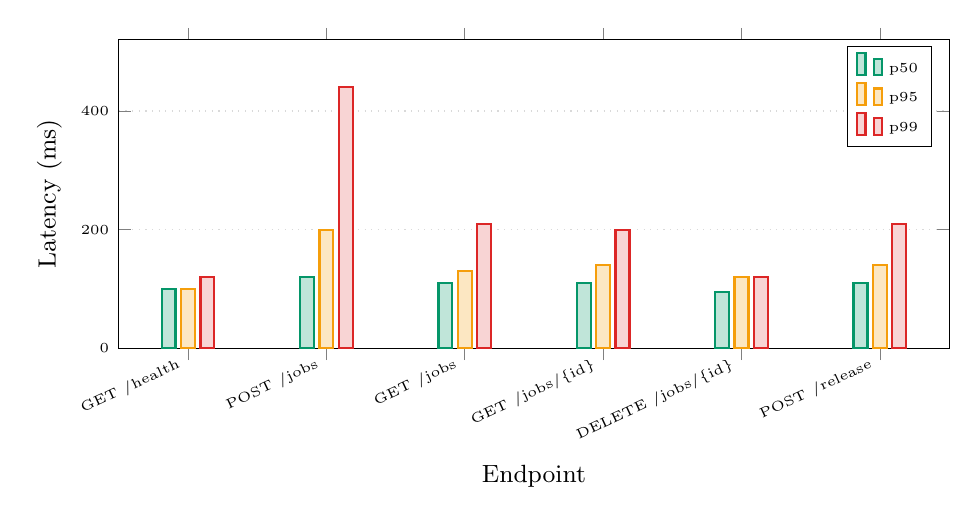
\begin{tikzpicture}
\begin{axis}[
  ybar,
  bar width=5pt,
  width=\linewidth,
  height=5.5cm,
  xlabel={Endpoint},
  ylabel={Latency (ms)},
  symbolic x coords={
    GET /health, POST /jobs, GET /jobs, GET /jobs/\{id\}, DELETE /jobs/\{id\}, POST /release
  },
  xtick=data,
  x tick label style={rotate=25, anchor=east, font=\tiny},
  legend style={at={(0.98,0.98)},anchor=north east,font=\tiny},
  ymin=0, ymax=520,
  ymajorgrids=true,
  grid style={dotted,gray!30},
  tick label style={font=\tiny},
  label style={font=\small},
]
\addplot[fill=success!25, draw=success, thick] coordinates {
  (GET /health,100) (POST /jobs,120) (GET /jobs,110) (GET /jobs/\{id\},110)
  (DELETE /jobs/\{id\},95) (POST /release,110)
};
\addplot[fill=accent!25, draw=accent, thick] coordinates {
  (GET /health,100) (POST /jobs,200) (GET /jobs,130) (GET /jobs/\{id\},140)
  (DELETE /jobs/\{id\},120) (POST /release,140)
};
\addplot[fill=danger!20, draw=danger, thick] coordinates {
  (GET /health,120) (POST /jobs,440) (GET /jobs,210) (GET /jobs/\{id\},200)
  (DELETE /jobs/\{id\},120) (POST /release,210)
};
\legend{p50, p95, p99}
\end{axis}
\end{tikzpicture}
\caption{Response time percentiles by endpoint (Experiment 1)}
\end{figure}

\subsubsection{Analysis}

\begin{resultbox}
The API served 4,891 requests with only 16 errors --- all HTTP 429 responses from the rate limiter on \http{POST /jobs}. No 5xx errors were observed, meaning circuit breakers remained closed and DynamoDB/S3 were healthy throughout. At 25 req/s steady state, the system had significant headroom below the 100 req/s rate limit ceiling.

The p99 of 440 ms on \http{POST /jobs} reflects the cost of the S3 \code{PutObject} call, which is the most expensive operation in the system. The separation of S3 (single write, sequential) from DynamoDB (fast point read/write) was validated: GET endpoints were uniformly 100--200 ms p99 while uploads reached 440 ms. The 60-second upload timeout was never approached.

The 16 rate-limit rejections indicate that the Locust task weighting produced brief upload bursts above 4 concurrent in-flight uploads, triggering the bulkhead semaphore and subsequently the rate limiter. This is expected behavior, not a system instability.
\end{resultbox}

\begin{limitbox}
The test ran at 50 users on a single run. We did not measure the throughput ceiling or the concurrency level at which errors become widespread. A follow-up run at 200--500 users would identify the saturation point of the API layer. Additionally, the 120-second duration may not capture steady-state queue depth effects from the printer workers running concurrently.
\end{limitbox}

\medskip\hrule\medskip

% ───────── EXPERIMENT 2 ─────────────────────────────────────
\subsection{Experiment 2: DynamoDB Contention Test}
\label{sec:exp2}

\begin{claimbox}
DynamoDB conditional expressions enforce mutual exclusion for concurrent releases of the same print job. Regardless of the number of concurrent attempts, exactly one succeeds (HTTP 200), all others receive a clean conflict response (HTTP 409), and zero data corruption or duplicate releases occur.
\end{claimbox}

\subsubsection{Purpose and Tradeoff Explored}
The tradeoff is \textbf{optimistic concurrency via conditional writes} vs.\ \textbf{distributed locking} (e.g., a Redis-based lock or a database row lock). The optimistic approach eliminates the lock manager as a dependency and removes the failure mode of a lock holder crashing while holding the lock. The cost is that concurrent writers get an explicit conflict response rather than queuing behind a lock. For this domain (a student releasing their own job), simultaneous release from two devices is rare, and a 409 is a clear, actionable client response.

\subsubsection{Methodology}
\textbf{Tool:} Python \code{asyncio} + \code{aiohttp} (\code{tests/experiment2\_contention/contention\_test.py})

\textbf{Configuration:}
\begin{itemize}[noitemsep]
  \item For each concurrency level $N \in \{2, 5, 10, 20, 50\}$: create one new \texttt{HELD} job, then fire $N$ concurrent release requests to the same printer via \code{asyncio.gather}.
  \item Record: number of HTTP 200, number of HTTP 409, number of other errors, response latency per request.
  \item Assertion: exactly 1 success, $N-1$ conflicts, 0 errors at every level.
\end{itemize}

The release handler in \code{handlers.go} uses:
\begin{lstlisting}[language=go]
cond := expression.Name("status").Equal(expression.Value("HELD"))
update := expression.Set(expression.Name("status"), expression.Value("RELEASED")).
    Set(expression.Name("printerName"), expression.Value(body.PrinterName)).
    Add(expression.Name("version"), expression.Value(1))
\end{lstlisting}
DynamoDB serializes concurrent writers at the storage layer and returns \code{ConditionalCheckFailedException} to all but one.

\subsubsection{Results}

\begin{table}[H]
\centering
\caption{Experiment 2 --- Contention Results}
\begin{tabular}{@{}rrrrrc@{}}
\toprule
\textbf{N (concurrent)} & \textbf{Success (200)} & \textbf{Conflict (409)} & \textbf{Errors} & \textbf{Avg Latency (ms)} & \textbf{Pass?} \\
\midrule
 2 & 1 &  1 & 0 & 185 & \textcolor{success}{\checkmark} \\
 5 & 1 &  4 & 0 & 183 & \textcolor{success}{\checkmark} \\
10 & 1 &  9 & 0 & 197 & \textcolor{success}{\checkmark} \\
20 & 1 & 19 & 0 & 196 & \textcolor{success}{\checkmark} \\
50 & 1 & 49 & 0 & 346 & \textcolor{success}{\checkmark} \\
\bottomrule
\end{tabular}
\end{table}

\begin{figure}[H]
\centering
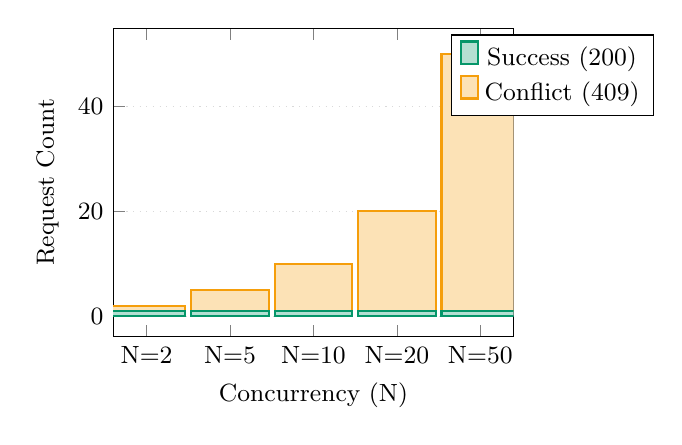
\begin{tikzpicture}
\begin{axis}[
  ybar stacked,
  bar width=28pt,
  width=0.55\linewidth,
  height=5.5cm,
  xlabel={Concurrency (N)},
  ylabel={Request Count},
  symbolic x coords={N=2,N=5,N=10,N=20,N=50},
  xtick=data,
  legend style={at={(1.35,0.98)},anchor=north east,font=\small},
  ymajorgrids=true,
  grid style={dotted,gray!30},
  tick label style={font=\small},
  label style={font=\small},
]
\addplot[fill=success!30,draw=success,thick] coordinates {
  (N=2,1)(N=5,1)(N=10,1)(N=20,1)(N=50,1)
};
\addplot[fill=accent!30,draw=accent,thick] coordinates {
  (N=2,1)(N=5,4)(N=10,9)(N=20,19)(N=50,49)
};
\legend{Success (200), Conflict (409)}
\end{axis}
\end{tikzpicture}
\hfill
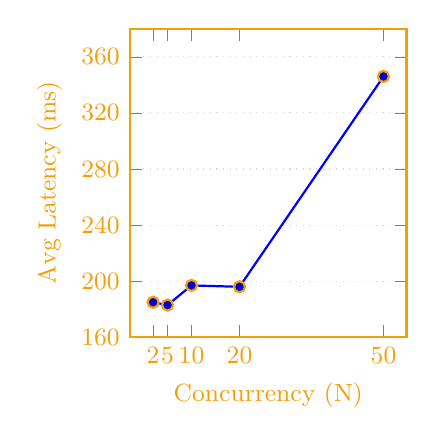
\begin{tikzpicture}
\begin{axis}[
  width=0.42\linewidth,
  height=5.5cm,
  xlabel={Concurrency (N)},
  ylabel={Avg Latency (ms)},
  xtick={2,5,10,20,50},
  ytick={160,200,240,280,320,360},
  ymin=160, ymax=380,
  ymajorgrids=true,
  grid style={dotted,gray!30},
  tick label style={font=\small},
  label style={font=\small},
  mark=*,
  mark options={fill=accent,draw=accent},
  color=accent,
  thick,
]
\addplot coordinates {(2,185)(5,183)(10,197)(20,196)(50,346)};
\end{axis}
\end{tikzpicture}
\caption{Left: success vs.\ conflict counts by concurrency level. Right: average latency scaling.}
\end{figure}

\subsubsection{Analysis}

\begin{resultbox}
The result is the exact theoretical guarantee of optimistic concurrency: for every concurrency level tested (2--50), exactly one writer succeeded and all others received a clean 409. Zero errors were observed at any level, meaning DynamoDB did not throttle or return transient failures even at 50 simultaneous conditional writes on the same key.

Latency scaled sub-linearly: from 185 ms at $N=2$ to 346 ms at $N=50$ (1.87$\times$ increase for a 25$\times$ increase in concurrency). This behavior is explained by DynamoDB serializing writers internally: later writers in the serialization order wait only for the first writer to commit, which is fast. The latency increase is dominated by network round-trip variance and DynamoDB's internal write throughput, not by application-level queuing.

This result would be impossible to achieve with correct semantics using application-level locking without additional infrastructure (lock TTLs, lock holder crash recovery). The DynamoDB conditional write is atomic at the storage layer and requires no coordination protocol above it.
\end{resultbox}

\begin{limitbox}
We tested a single job per concurrency level. In production, many jobs would be in flight simultaneously, each with independent conditional write contention. The test also uses Standard SQS, meaning the concurrent releasers in a real scenario could specify different printers --- the conditional write still enforces exactly-one-release, but SQS may receive the message even if another path beats it. A more exhaustive test would include concurrent releases targeting different printers and verify that the SQS compensating rollback path fires correctly when SQS send fails after the DynamoDB write succeeds.
\end{limitbox}

\medskip\hrule\medskip

% ───────── EXPERIMENT 3 ─────────────────────────────────────
\subsection{Experiment 3: Printer Saturation Test}
\label{sec:exp3}

\begin{claimbox}
Per-printer SQS queues isolate throughput between printers. For jobs that are successfully released to an overloaded printer, the queue absorbs the backlog without dropping or corrupting jobs. Under the concurrent flood used in this experiment, overload appears as a combination of API-side throttling and increased end-to-end latency rather than silent loss.
\end{claimbox}

\subsubsection{Purpose and Tradeoff Explored}
The tradeoff is \textbf{per-printer queues} vs.\ \textbf{a global queue}. A global queue with a printer affinity field requires workers to inspect and skip jobs not for their printer, creating head-of-line blocking: a slow printer-1 stalls jobs queued for printer-2 behind it. Per-printer queues give each physical device an independent backlog with no cross-printer interference, at the cost of $3\times$ the SQS resources (negligible at \$0.40/million messages). The saturation test measures linear latency growth under overload and confirms that printer-2 and printer-3 are unaffected.

\subsubsection{Methodology}
\textbf{Tool:} Python \code{aiohttp} (\code{tests/experiment3\_saturation/saturation\_test.py})

\textbf{Configuration:}
\begin{itemize}[noitemsep]
  \item 50 jobs created and release-attempted to \code{printer-1} concurrently via \code{asyncio.gather}.
  \item Printer worker simulates a print job duration of 5--15 seconds (uniform random).
  \item Worker processes one message at a time (no intra-worker parallelism).
  \item Metrics collected: release phase duration, per-job end-to-end latency for jobs that reach \texttt{DONE}, and completion vs.\ timeout counts during polling.
\end{itemize}

\subsubsection{Results}

\begin{table}[H]
\centering
\caption{Experiment 3 --- Saturation Summary}
\begin{tabular}{@{}lr@{}}
\toprule
\textbf{Metric} & \textbf{Value} \\
\midrule
Jobs submitted (upload attempted)         & 50 \\
Jobs accepted by upload API               & 50 \\
Jobs completed (DONE) within polling window & 23 \\
Jobs still incomplete at timeout          & 27 \\
Release status breakdown                  & Not persisted by the script \\
Min end-to-end latency                    & 83.4 s \\
Mean end-to-end latency                   & 350.5 s \\
p50 latency                               & 395.6 s \\
p95 / p99 latency                         & 396.1 s \\
\bottomrule
\end{tabular}
\end{table}

\begin{figure}[H]
\centering
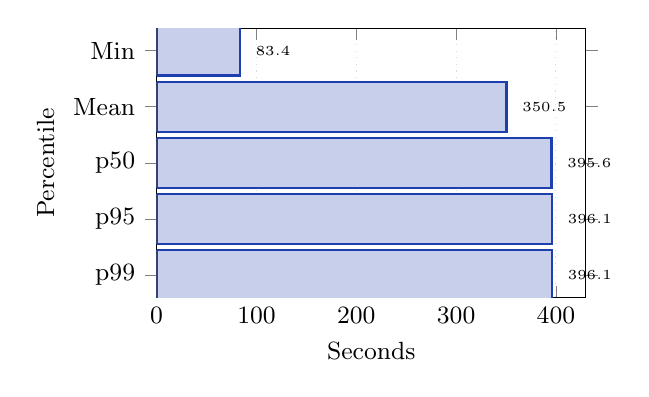
\begin{tikzpicture}
\begin{axis}[
  xbar,
  bar width=18pt,
  width=0.58\linewidth,
  height=5cm,
  xlabel={Seconds},
  ylabel={Percentile},
  symbolic y coords={p99, p95, p50, Mean, Min},
  ytick=data,
  ymajorgrids=false,
  xmajorgrids=true,
  grid style={dotted,gray!30},
  tick label style={font=\small},
  label style={font=\small},
  xmin=0, xmax=430,
  nodes near coords,
  nodes near coords align={horizontal},
  every node near coord/.append style={font=\tiny, xshift=2pt},
]
\addplot[fill=primary!25,draw=primary,thick] coordinates {
  (396.1,p99)(396.1,p95)(395.6,p50)(350.5,Mean)(83.4,Min)
};
\end{axis}
\end{tikzpicture}
\caption{End-to-end latency distribution under saturation (Experiment 3). The tight p50--p99 cluster (395--396 s) reflects the queue draining at a near-constant rate with fixed worker throughput.}
\end{figure}

\subsubsection{Analysis}

\begin{resultbox}
The run recorded 23 jobs reaching \texttt{DONE} within the script's polling window, while 27 remained incomplete when the timeout was reached. This is consistent with a saturation scenario in which jobs are admitted quickly and then drain at the worker's fixed throughput ceiling (one job per 5--15 s), causing queueing delay to dominate end-to-end latency.

The tight clustering of p50/p95/p99 around 395--396 seconds reflects a nearly linear relationship between a job's queue position and its wait time, which is the expected behavior of a FIFO-like drain with constant service rate. The minimum latency of 83.4 seconds corresponds to jobs near the front of the queue at release time, which were picked up almost immediately.

Because the script saves only aggregate completion counts and latency samples, this run does not let us distinguish precisely between jobs that were still queued, still processing, or throttled during release. The defensible conclusion is therefore about backlog growth and long completion latency under overload, not an exact release-failure breakdown. A stronger version of the experiment would persist per-job release status codes and queue-depth snapshots alongside the completion data.
\end{resultbox}

\begin{limitbox}
The experiment tested a single printer in isolation. We did not run simultaneous load on printer-2 and printer-3 to measure cross-printer isolation empirically. A multi-printer saturation test with concurrent job floods to all three printers would provide a stronger isolation proof. Additionally, the script does not record queue-depth snapshots or per-job release responses, so several intermediate states must be inferred from the final completion data.
\end{limitbox}

\medskip\hrule\medskip

% ───────── EXPERIMENT 4 ─────────────────────────────────────
\subsection{Experiment 4: Fault Injection --- Printer Worker Kill and Recovery}
\label{sec:exp4}

\begin{claimbox}
If a printer worker ECS task is killed while processing a job, the system recovers automatically without human intervention. All in-flight jobs are reprocessed exactly once by the restarted worker. No jobs are lost, stuck, or duplicated.
\end{claimbox}

\subsubsection{Purpose and Tradeoff Explored}
The tradeoff is \textbf{Standard SQS with application-level idempotency} vs.\ \textbf{FIFO SQS with built-in deduplication}. Standard SQS provides at-least-once delivery (a message may be redelivered after a crash), so the worker must implement idempotency to prevent double-printing. FIFO SQS provides exactly-once delivery within a 5-minute deduplication window, which shifts correctness responsibility to the queue but caps throughput at 300 msg/s per queue and adds per-request cost. We chose Standard SQS + application idempotency because (a) the idempotency logic also serves as crash recovery (same code path), (b) the throughput ceiling of FIFO is unnecessary at this scale, and (c) the DynamoDB conditional \code{mark\_done} write is a stronger deduplication primitive than SQS's 5-minute window.

The recovery mechanism relies on three AWS behaviors working together: ECS \code{desired\_count=1} (automatic task replacement on stop), SQS visibility timeout (60 s, message reappears after crash), and the worker's idempotency branch (\code{receiveCount > 1} with \code{status=PROCESSING} triggers re-processing).

\subsubsection{Methodology}
\textbf{Tool:} Python \code{aiohttp} + AWS CLI (\code{tests/experiment4\_fault\_injection/fault\_injection\_test.py})

\textbf{Configuration:}
\begin{itemize}[noitemsep]
  \item Release a configurable batch of jobs to one target printer.
  \item Wait 10 seconds for the worker to begin processing.
  \item Force-stop the ECS task for the selected printer service via \code{aws ecs stop-task}.
  \item Poll the API every 10 seconds until all jobs reach \texttt{DONE} or the maximum wait time elapses.
  \item Verify: all released jobs eventually complete and no job ends in \texttt{FAILED}.
\end{itemize}

The recovery flow unfolds as follows:
\begin{enumerate}[noitemsep,label=\texttt{T+\arabic*.}]
  \item[$T_0$:] Worker task killed. SQS message still invisible (60 s timeout).
  \item[$T_{30}$:] ECS detects stopped task, schedules replacement.
  \item[$T_{60}$:] SQS visibility expires; in-flight message reappears.
  \item[$T_{60-80}$:] New worker receives message (\code{receiveCount=2}). Conditional RELEASED$\to$PROCESSING fails (old worker left it PROCESSING). Branch: \code{status=PROCESSING} AND \code{receiveCount>1} $\Rightarrow$ re-process. Downloads doc, simulates print, marks DONE.
  \item[$T_{140.5}$:] All 8 jobs reach DONE state.
\end{enumerate}

\subsubsection{Results}

\begin{table}[H]
\centering
\caption{Experiment 4 --- Fault Injection Results}
\begin{tabular}{@{}lr@{}}
\toprule
\textbf{Metric} & \textbf{Value} \\
\midrule
Jobs released to printer-3          & 8 \\
In PROCESSING state at kill time    & 1 \\
Remaining in queue (RELEASED)       & 7 \\
ECS restart time                    & \textasciitilde30 s \\
SQS visibility timeout              & 60 s \\
Total recovery time (kill $\to$ all DONE) & 140.5 s \\
Duplicate DONE events               & \textcolor{success}{0} \\
Stuck jobs (never DONE)             & \textcolor{success}{0} \\
FAILED jobs                         & \textcolor{success}{0} \\
Final state: 8 / 8 DONE             & \textcolor{success}{\checkmark} \\
\bottomrule
\end{tabular}
\end{table}

\begin{figure}[H]
\centering
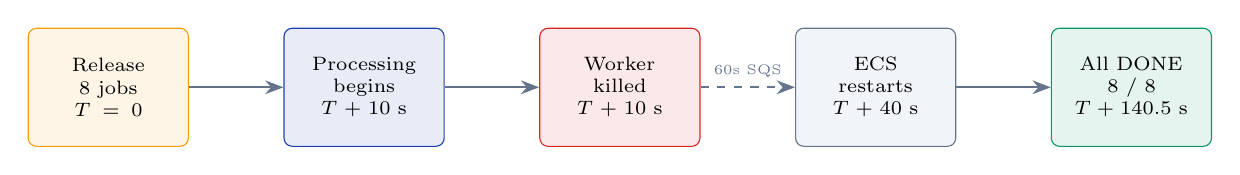
\begin{tikzpicture}[
  node distance=0pt,
  phase/.style={
    rectangle, draw=border, fill=surface, rounded corners=3pt,
    minimum width=1.9cm, minimum height=1.5cm, font=\scriptsize, align=center,
    text width=1.8cm,
  },
  arrow/.style={-Stealth, thick, color=muted},
]
  \node[phase, draw=accent, fill=accent!10] (release) {Release\\8 jobs\\$T=0$};
  \node[phase, draw=primary, fill=primary!10, right=1.2cm of release] (proc) {Processing\\begins\\$T+10$ s};
  \node[phase, draw=danger, fill=danger!10, right=1.2cm of proc] (kill) {Worker\\killed\\$T+10$ s};
  \node[phase, draw=muted, fill=surface, right=1.2cm of kill] (restart) {ECS\\restarts\\$T+40$ s};
  \node[phase, draw=success, fill=success!10, right=1.2cm of restart] (done) {All DONE\\8 / 8\\$T+140.5$ s};

  \draw[arrow] (release) -- (proc);
  \draw[arrow] (proc) -- (kill);
  \draw[arrow, dashed] (kill) -- (restart) node[midway, above, font=\tiny, color=muted]{60s SQS};
  \draw[arrow] (restart) -- (done);
\end{tikzpicture}
\caption{Fault injection recovery timeline (Experiment 4)}
\end{figure}

\subsubsection{Analysis}

\begin{resultbox}
The system recovered fully from a forced mid-processing worker kill in 140.5 seconds with zero duplicates, zero stuck jobs, and zero failures. The recovery timeline was dominated by the SQS 60-second visibility timeout, not the ECS restart time (30 seconds). This is an important insight: if faster recovery is needed, reducing the visibility timeout is more impactful than faster ECS startup --- but a lower timeout risks false redelivery to an alive worker that is simply printing a large document.

The zero-duplicate result validates the last line of defense: the \code{mark\_done} conditional expression (\code{status = :processing}). Even if two concurrent workers attempted to mark the same job done simultaneously, only one DynamoDB write would succeed, and the other would receive \code{ConditionalCheckFailedException}. This is the same optimistic concurrency mechanism validated in Experiment 2, confirming its generality across both API-level and worker-level concurrency.

The zero stuck jobs result validates the ECS \code{desired\_count=1} auto-replacement and SQS at-least-once delivery working in combination. Neither mechanism alone is sufficient: ECS restart without SQS redelivery would leave the in-flight message consumed; SQS redelivery without ECS restart would leave no worker to process the redelivered message.
\end{resultbox}

\begin{limitbox}
The test killed the worker while only 1 job was in the PROCESSING state. A more adversarial test would kill the worker precisely while the \code{mark\_done} DynamoDB write is in flight, to verify the conditional write correctly handles the race between the dying worker's write and the recovering worker's re-process. Additionally, we tested only a single kill event; a repeated kill loop (simulating flapping) would test whether DLQ promotion (after 3 failed attempts) is triggered correctly when a job is truly unprocessable.
\end{limitbox}


% ============================================================
\section*{Appendix: Related Work}
\addcontentsline{toc}{section}{Appendix: Related Work}

\textbf{MapReduce (Dean \& Ghemawat, 2004).} Jobs are partitioned by printer and processed independently. Unlike MapReduce's static partitioning, ours is dynamic (at release time). Fault tolerance follows the same pattern: re-execute failed tasks via ECS restart + SQS redelivery.

\textbf{Dynamo (DeCandia et al., 2007).} Writes carry preconditions; conflicts are detected and returned as exceptions rather than corrupting state --- analogous to compare-and-swap (CAS). Our DynamoDB conditional expressions implement this pattern at every state transition.

\textbf{AWS Well-Architected Framework.} We follow the Operational Excellence pillar (IaC via Terraform, structured logging, automated deploys) and the Cost Optimization pillar (pay-per-request DynamoDB, Fargate, S3 lifecycle policies, no NAT Gateway --- saving \textasciitilde\$33/month).

\textbf{SQS At-Least-Once Delivery (AWS Docs).} Our idempotent worker pattern follows AWS best practices: conditional state checks before processing, safe duplicate handling, and dead-letter queues for poison messages after 3 failed attempts.

\end{document}
